\section{Конструкторская часть}

\subsection{Проектирование системы}

Верхнеуровневая диаграмма представлена на рисунке \ref{img:idef0}. На вход система получает данные о процессах документа и на выходе формирует результат моделирования исходя из статусной модели документа.

\begin{figure}[h!]
	\begin{center}
		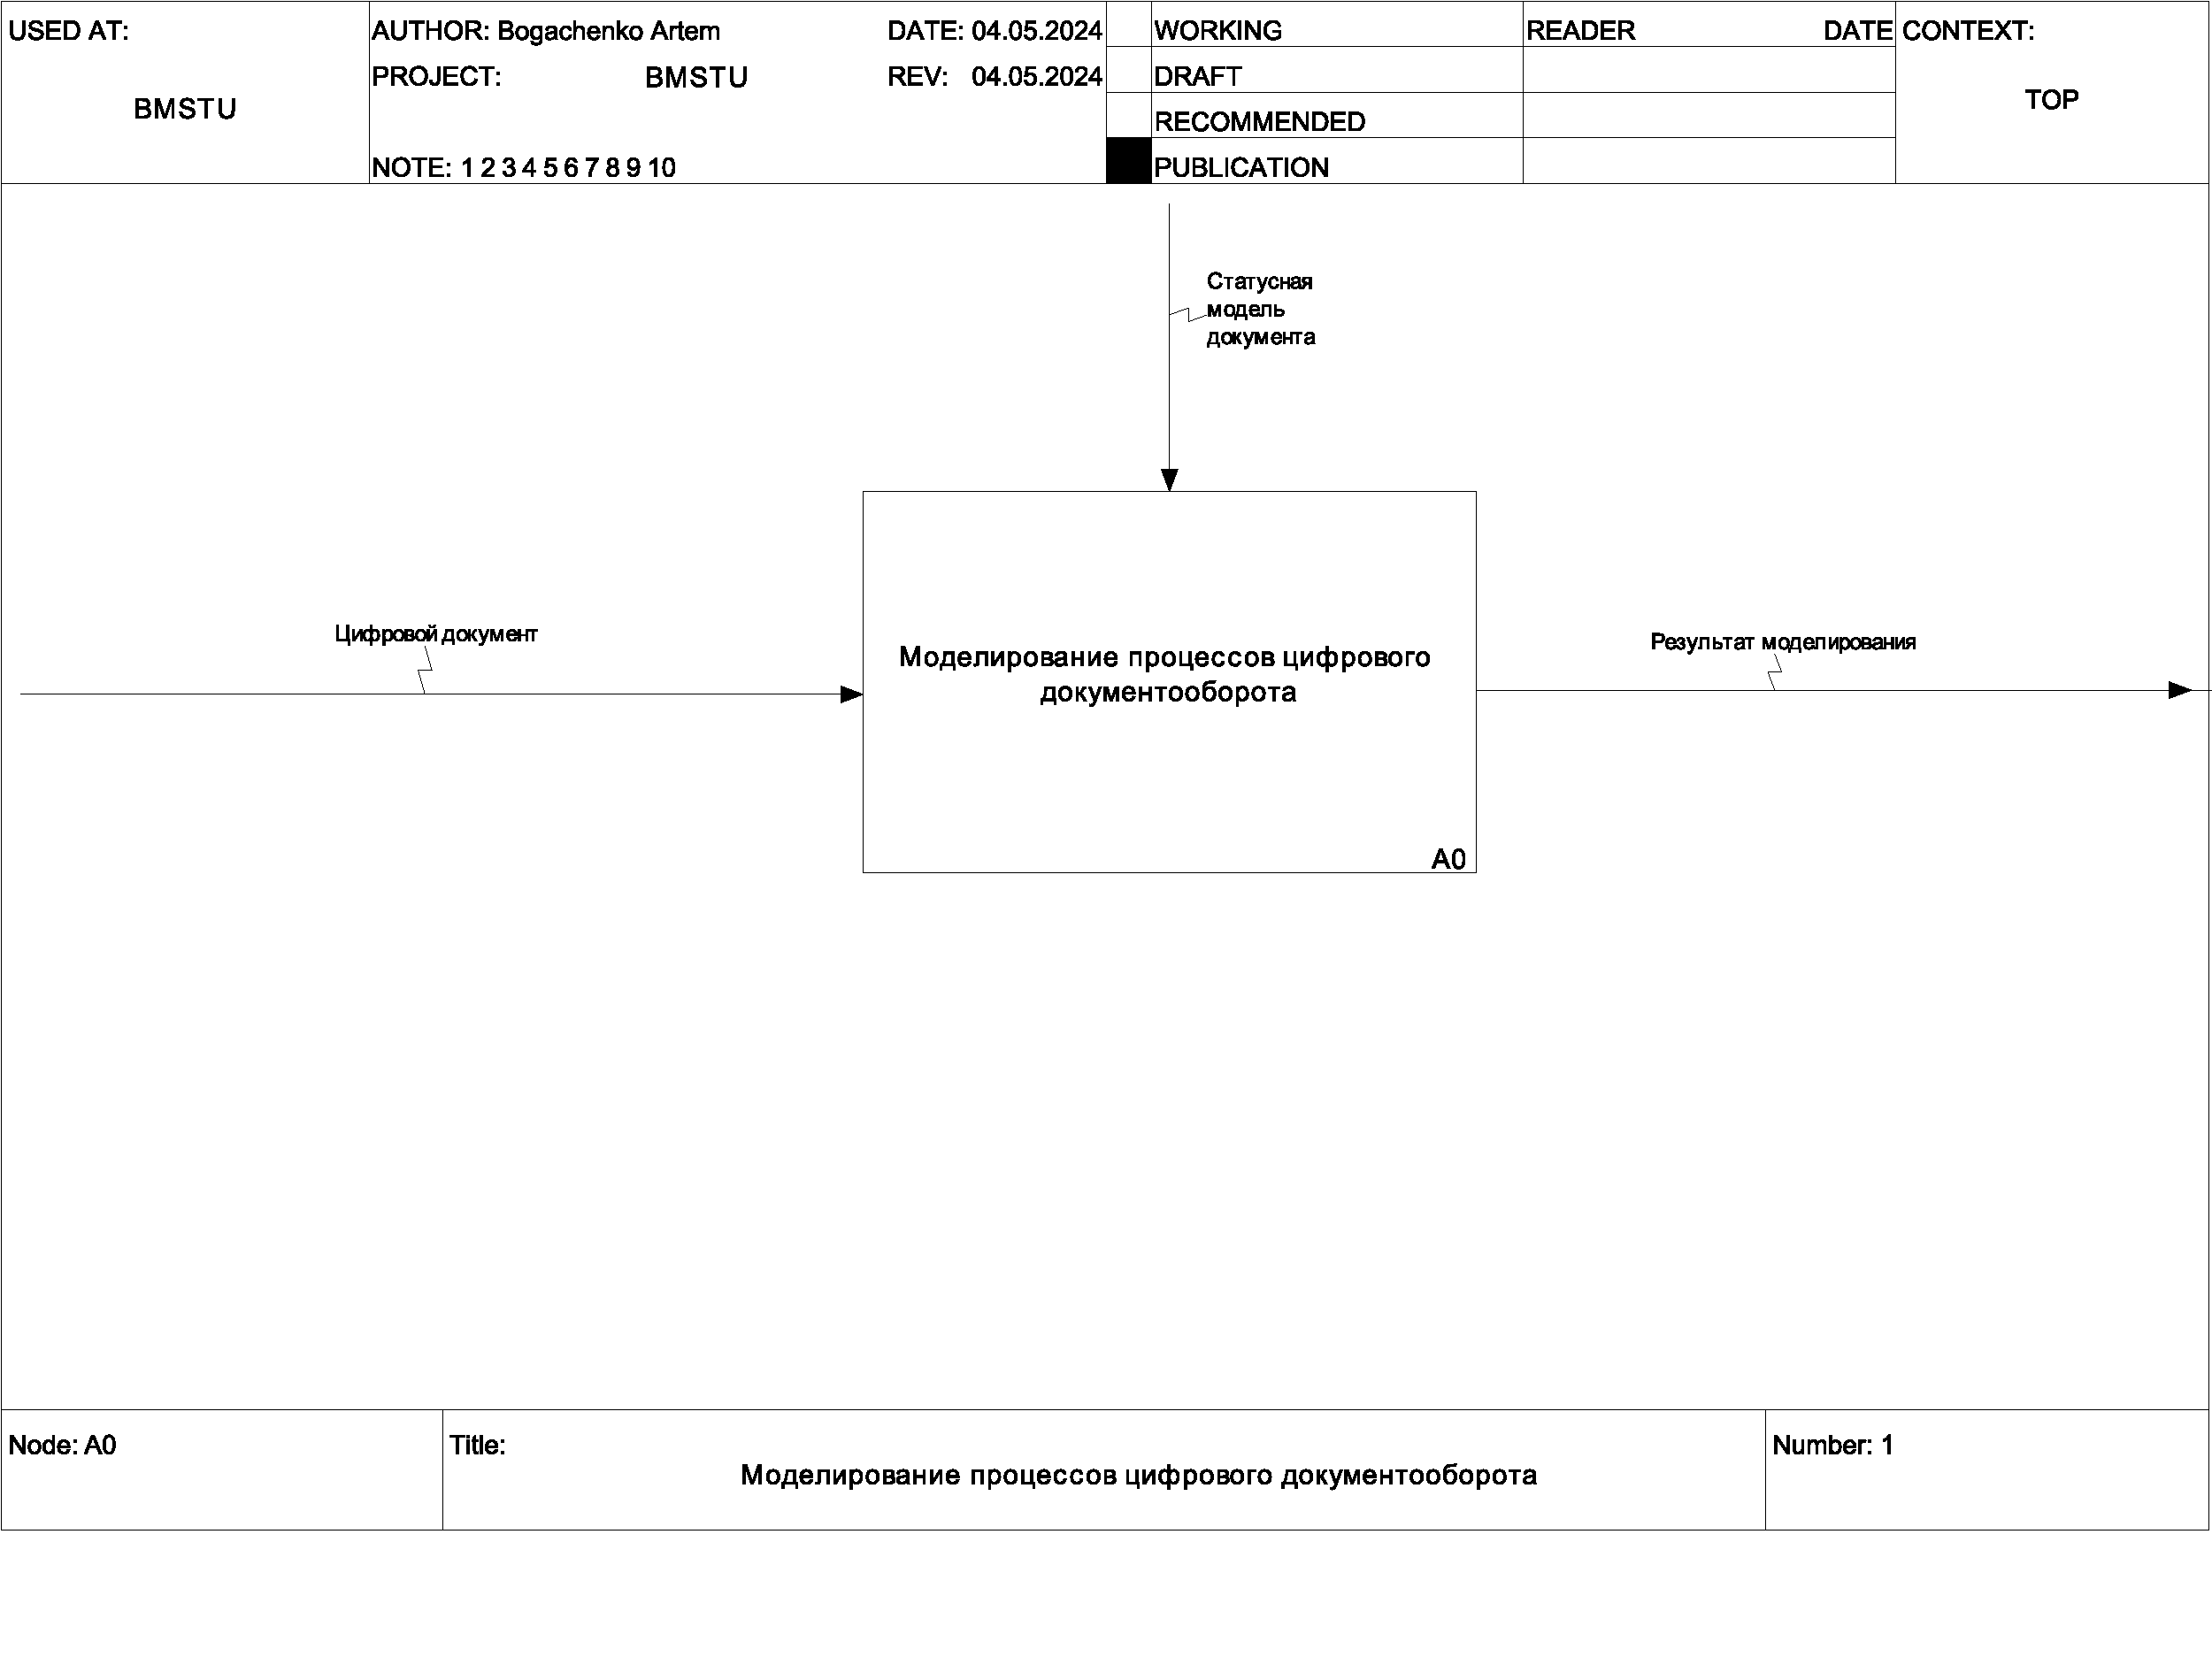
\includegraphics[scale=0.3666]{inc/idef0.pdf}
	\end{center}
	\captionsetup{justification=centering}
	\caption{Верхнеуровневая диаграмма приложения}
	\label{img:idef0}
\end{figure}

Результатом моделирования в данном случае являются временные границы прохождения документа по статусной модели и вероятность данного события.

\subsection{Проектирование алгоритма с использованием sTPN}

Для моделирование с помощью стохастической сети Петри необходимо программное обеспечение, позволяющее построить сеть Петри в соответствие со спецификой процессов определённого документа. Данное программное обеспечение должно предоставлять возможность введения стохастического перехода между местами в сети, определяющими статусы документа в соответствии со статусной моделью. Для проведения моделирование необходима возможно проведение прямого и обратного переходного анализа сети. Для интерпретации полученных результатов необходимо визуализация.
\subsection{Проектирование алгоритма с использованием квантового моделирования}

Аналогично концепции квантовых шахмат, размерность игрового поля при моделировании процессов цифрового документооборота будет зависеть от количества статусов, предусмотренных статусной моделью документа, от $1$ до $N$. В качестве фигуры будет документ. Ход совершается перемещением документа из одного статуса в другой. Формула вероятности хода для шахмат \ref{eq:chessprob} справедлива и для подсчёта вероятности перехода документа из одного статуса в другой. Для расчёта <<пути>> документа $D$, остаётся неизменной формула стандартного хода \ref{eq:chessstandard}, с единственным убранным ограничением на фигуры $v_s \in \{D\}$, ввиду того, что единственно-возможной фигурой в данном случае является сам документ и только он:

\begin{equation}\label{eq:docstandard}
	P_D = (v_s \in \{D\}) \wedge valid(t,s,v_s) \wedge ((v_t = 0) \vee (v_t = v_s)).
\end{equation}

Путь документа представлен на рисунке \ref{fig:doc2d}.

\begin{figure}[h!btp]
	\centering
	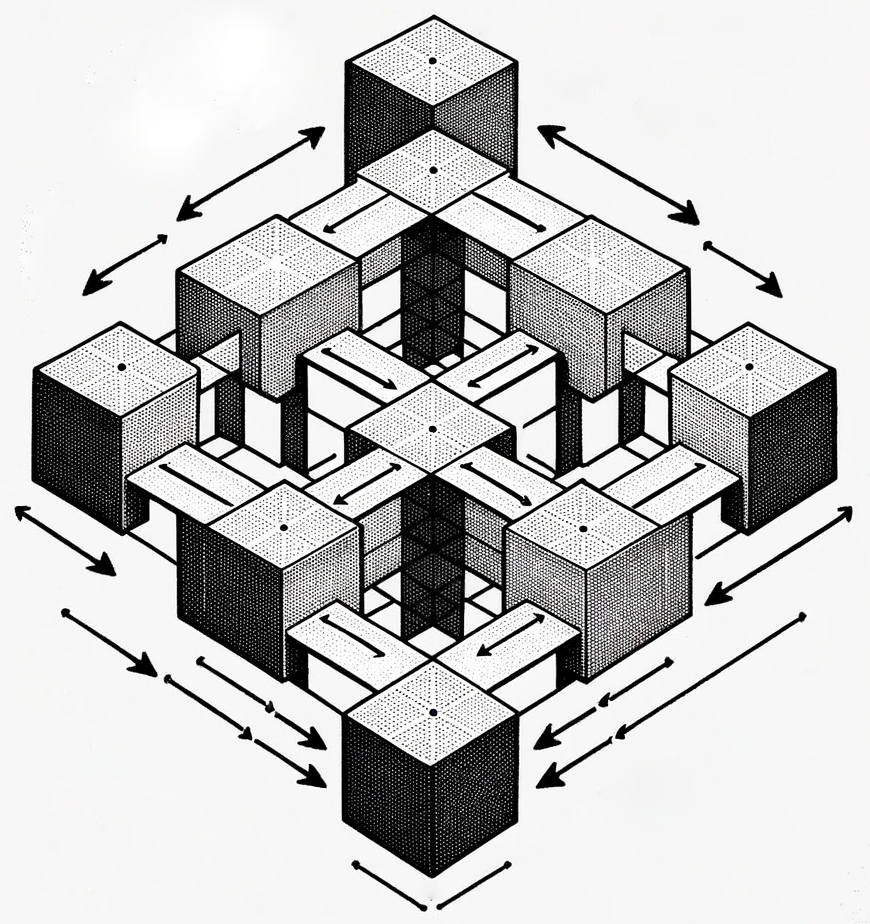
\includegraphics[width=0.55\textwidth]{inc/docv1.png}
	\caption{Визуализация пути документа}
	\label{fig:doc2d}
\end{figure}

\clearpage

\subsection{Схема алгоритма расчёта вероятностей}

Схема алгоритма подсчёта вероятностей представлена на рисунке \ref{fig:prolog}.

\begin{figure}[h!btp]
	\centering
	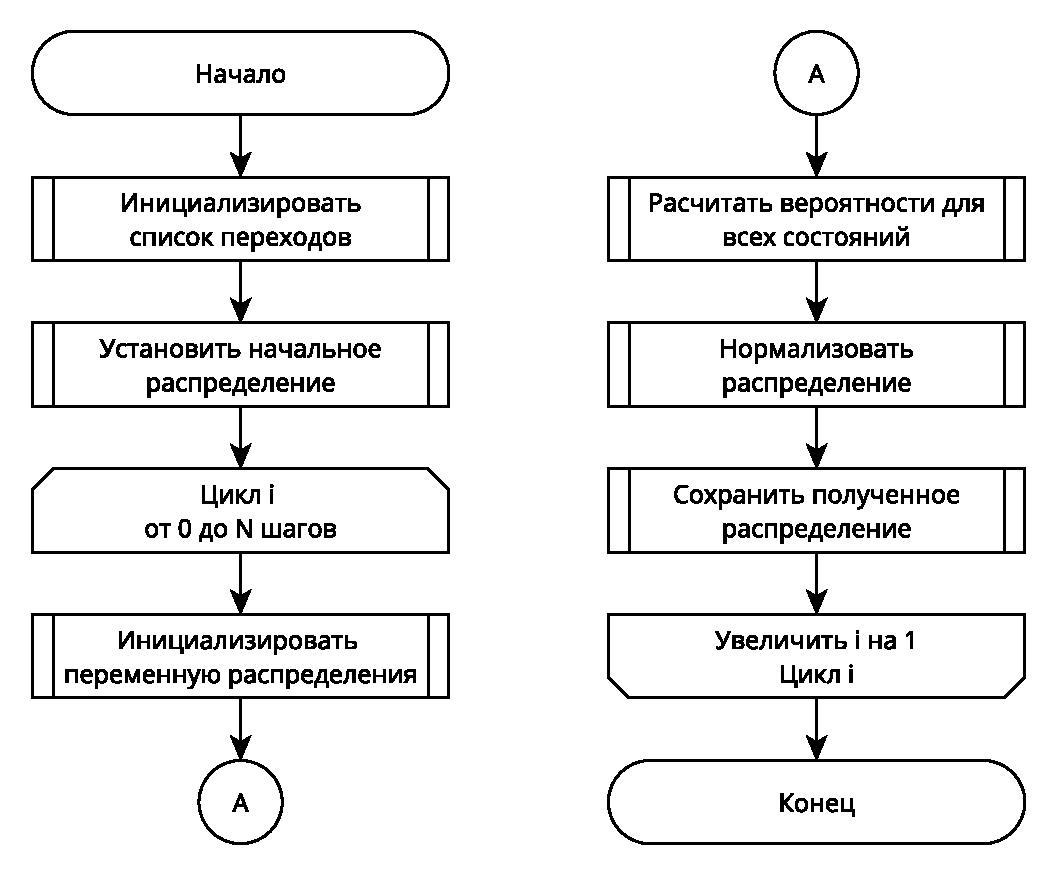
\includegraphics[width=0.55\textwidth]{inc/prolog.pdf}
	\caption{Схема алгоритма подсчёта вероятностей}
	\label{fig:prolog}
\end{figure}

\clearpage